\section{Clustering par partionement}
Nous avons réalisé le clustering par partitionnement en mettant en place deux méthodes : hierarchique et non hierarchique. 

\subsection{Santé}

\paragraph{Hierarchique}
Nous avons utilisé le composant hierarchical Clustering avec la configuration Linkage type : COMPLETE. Pour observer les résultats nous avons utilisé le composant Scatter Matrix.
Nous avions choisi de faire 3 clusters (cf section précédente), dont la répartitions des pays se fait comme suit : 

\begin{figure}[H]
	\begin{center}
		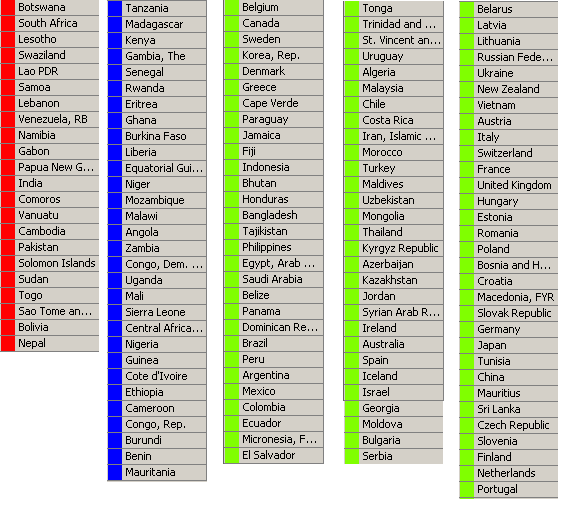
\includegraphics[scale=0.5]{Image/TableViewSanteNoMissing2}
		\caption{Liste des pays par clusters sur les critères de santé avec le jeu \jeuc}
	\end{center}
\end{figure}


Nous obtenons les résultats suivants : 

\begin{figure}[H]
	\begin{center}
		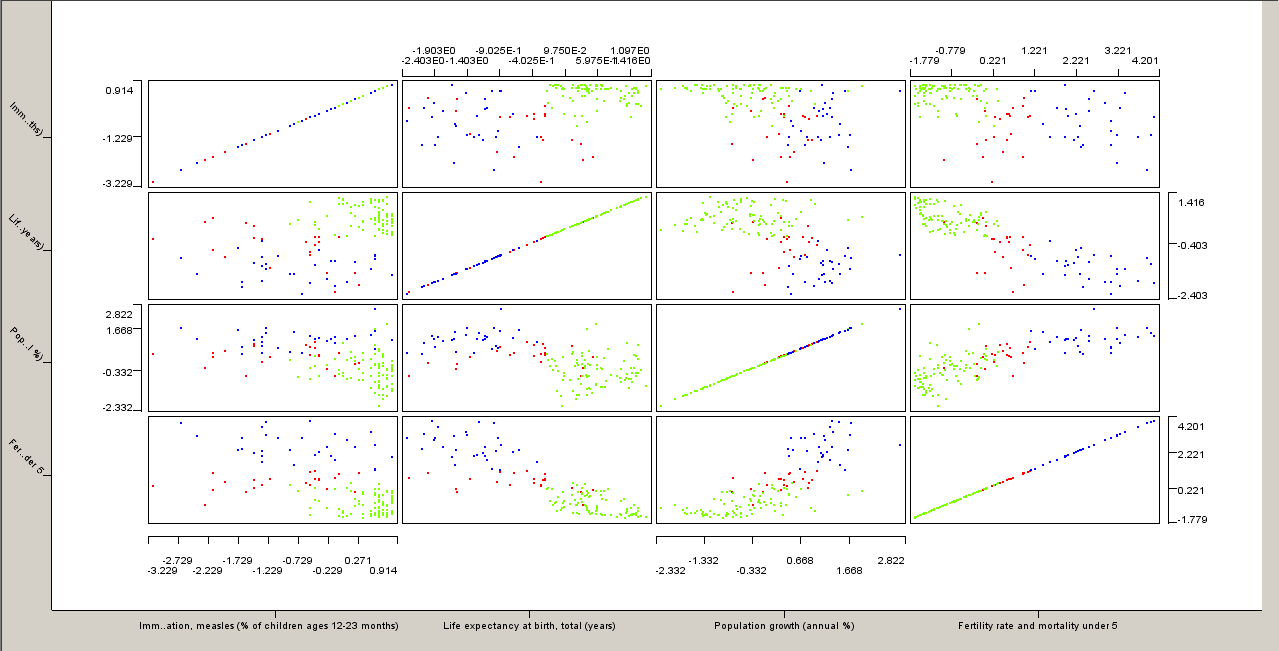
\includegraphics[scale=0.5]{Image/ScatterMatrixSanteNoMissing2}
		\caption{Scatter Matrix des attributs de l'indicateur Santé \jeuc}
	\end{center}
\end{figure}


\paragraph{Non Hierarchique}
L'application de K-means avec 99 itérations donne les clusters suivants: 

\begin{figure}[H]
	\begin{center}
		\includegraphics[scale=0.5]{Image/TableViewSanteKmeans}
		\caption{Liste des pays par clusters sur les critères de santé avec le jeu \jeuc}
	\end{center}
\end{figure}


Nous obtenons les résultats suivants : 

\begin{figure}[H]
	\begin{center}
		\includegraphics[scale=0.5]{Image/ScatterMatrixSanteKmeans}
		\caption{Scatter Matrix des attributs de l'indicateur Santé \jeuc}
	\end{center}
\end{figure}

K-means n'étant pas déterministe, nous devons vérifier sa stabilité.

\begin{Huge} 
scorer pour k-means 
\end{Huge}

\paragraph{Analyse}
Nous pouvons constater avec l'utilisation des deux méthodes de classification que nous avons une différence mais qu'elle n'est pas flagrante. Nous retrouvons les mêmes tendances.\\
Nous remarquons que nos clusters sont plus ou moins justifiable. En effet dans certain cas nous repérons bien 3 clusters distinct comme avec les attributs : Fertility rate and mortality under 5 et Life expectancy at birth. Mais cependant dans bon nombre de cas nous repérons plutôt un nuage de point très dispersés ou qui pourrait être modélisé comme une droite.\\
A la vue des représentations on constate que on aurait peut être du ne faire que deux clusters. Pour le moment nous ne pouvons pas conclure. Nous pouvons constater que le cluster vert est bien distinct du cluster bleu et que ces indicateurs de santé montrent de meilleures conditions  sanitaires.\\
Comme le montre le tableau plus haut nous remarquons que le cluster vert regroupe bon nombre de pays européen alors que le cluster bleu regroupe bon nombre de pays d'Afrique ce qui est un résultat pas cohérent en vue de ce que nous savons de l'état actuel de ces pays.


\subsection{Économie}
Au vu des distances obtenues dans la section précédente, nous obtenons 4 clusters.

\paragraph{Hierarchique} Par classification hiérarchique, nous obtenons les clusters suivants :

\begin{figure}[H]
	\begin{center}
		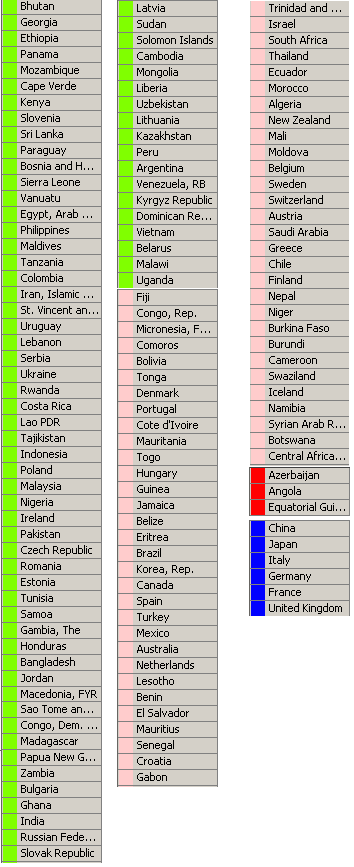
\includegraphics[scale=0.5]{Image/TableViewPolitiqueNoMissing2}
		\caption{Liste des pays par clusters sur les critères économiques avec le jeu \jeuc}
	\end{center}
\end{figure}


Nous obtenons les résultats suivants : 

\begin{figure}[H]
	\begin{center}
		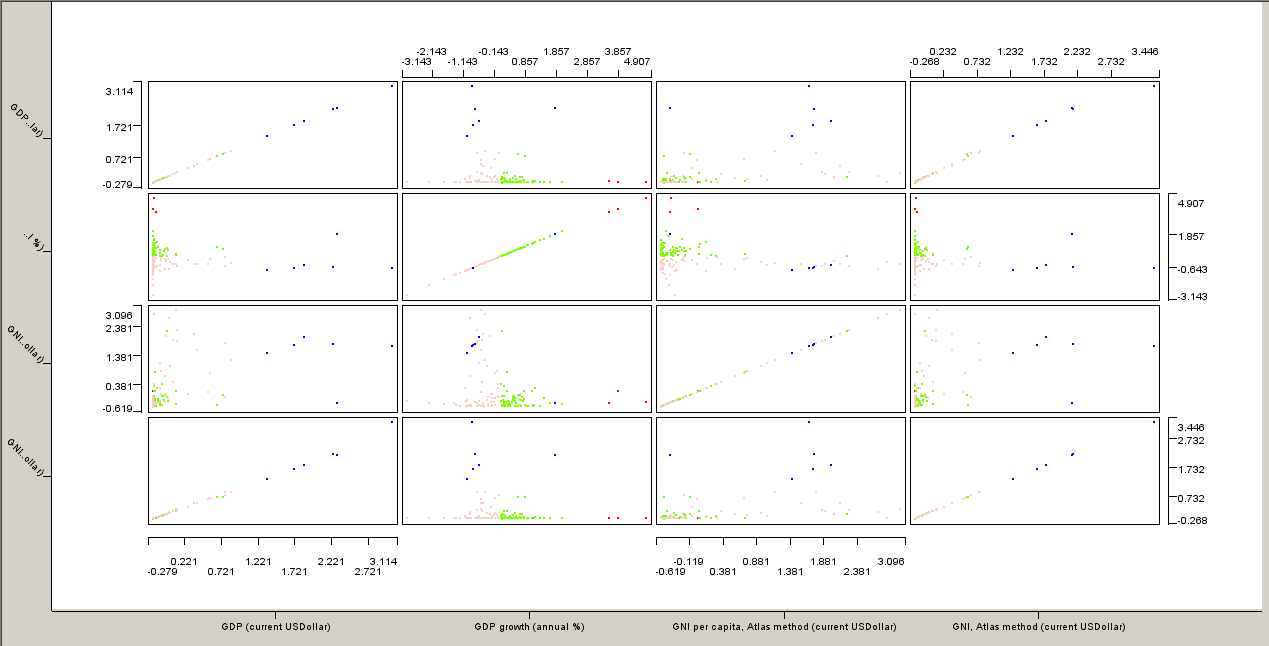
\includegraphics[scale=0.5]{Image/ScatterMatrixPolitiqueNoMissing2}
		\caption{Scatter Matrix des attributs de l'indicateur de politique économique \jeuc}
	\end{center}
\end{figure}

\paragraph{Non Hierarchique}
L'application de K-means donne les clusters suivants: 

\begin{figure}[H]
	\begin{center}
		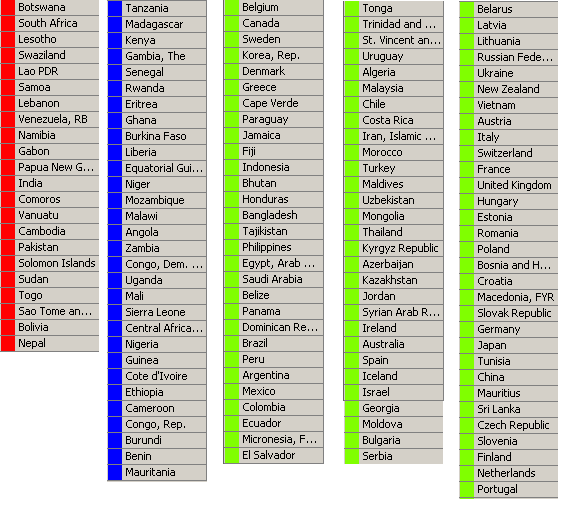
\includegraphics[scale=0.5]{Image/TableViewSanteNoMissing2}
		\caption{Liste des pays par clusters sur les critères de santé avec le jeu \jeuc}
	\end{center}
\end{figure}


Nous obtenons les résultats suivants : 

\begin{figure}[H]
	\begin{center}
		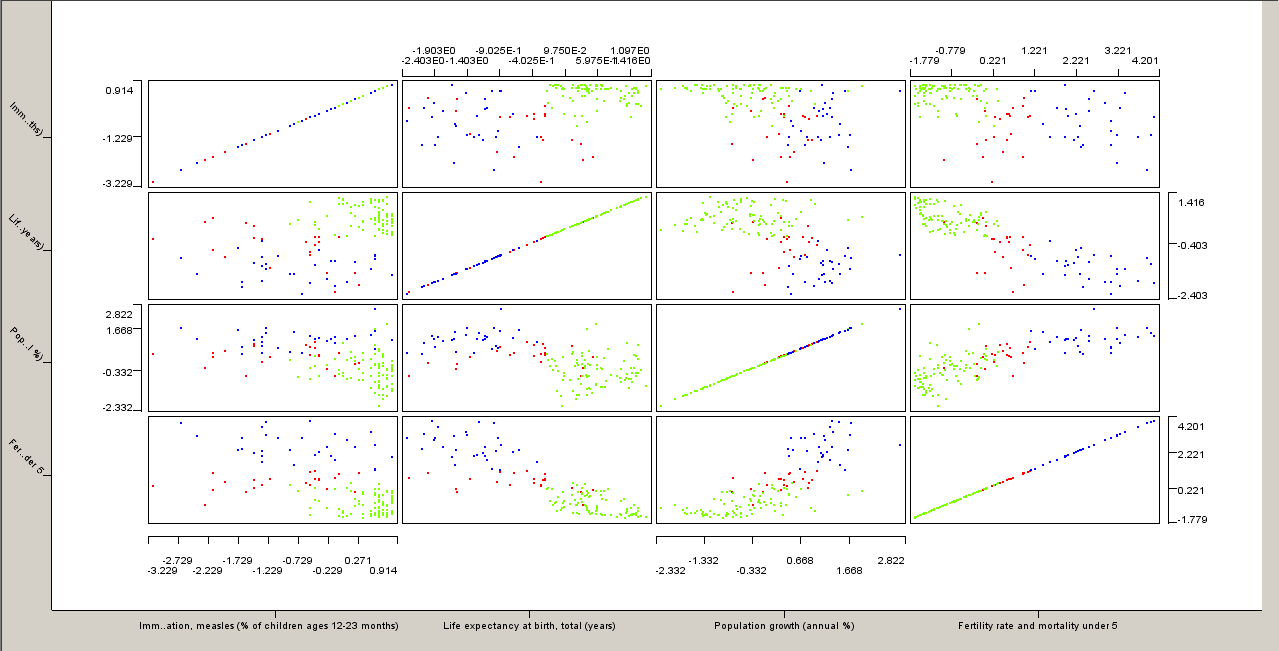
\includegraphics[scale=0.5]{Image/ScatterMatrixSanteNoMissing2}
		\caption{Scatter Matrix des attributs de l'indicateur Santé \jeuc}
	\end{center}
\end{figure}

K-means n'étant pas déterministe, nous devons vérifier sa stabilité.

\begin{Huge}


scorer pour k-means 
\end{Huge} 


\paragraph{Analyse}




